\documentclass[titlepage]{article}

\usepackage{tabularx}
\usepackage{booktabs}
\usepackage[bottom=3cm, right=3cm, left=3cm, top=3cm]{geometry}
\usepackage{graphicx}
\usepackage{hyperref}
\usepackage{float}
\newcommand\tab[1][1cm]{\hspace*{#1}}

\title{COMPSCI 4NL3: Natural Language Processing\\
Phase 3 Report}

\author{Team 4\\
\\ Junnan Li
\\ Nawaal Fatima
\\ Rashad Bhuiyan
\\ Sumanya Gulati}                  

\date{17 March 2025}

\begin{document}

\begin{titlepage}
  \maketitle
\end{titlepage}

\newpage

\tableofcontents

\newpage

\section{Annotation Analysis}
% How we computed agreement and how the metric was chosen
We computed agreement through the use of the Cohen's Kappa agreement metric. This metric is best used for pairwise agreement between two annotators. 
Since we split the data between 8 annotators with each annotator having some unique sample of a duplicated dataset within their task, this allows for 
duplicate annotation tasks to exist, making it viable to use Cohen's Kappa to calculate agreement. This is why we chose Cohen's Kappa as our preferred 
agreement metric. \\ 
\newline
We calculated the Cohen's Kappa agreement metric using the \textbf{cohen\_kappa\_score} method from the \textbf{sklearn.metrics} package. 
Since the annotations were binary in nature (either having positive-negative sentiment or team-individual focus), we would need to calculate two
separate Cohen-Kappa scores to ensure the reliability of our dataset: a Positive-Negative (Sentiment) Score, and a Team-Individual (Focus) Score.
We extracted the duplicate data from the combined dataset. Unfortunately, we had only 5\% of the duplications available due to a miscalculation of
proportions from phase 1, which could affect the reliability of the result as the sample size may seem too small. To combat this, we had our team 
members personally annotate certain datapoints in the dataset to introduce more duplicate data and included that as part of the full dataset.
The Cohen-Kappa scores for each agreement requirement is as follows:
\begin{itemize}
  \item Sentiment Cohen-Kappa Score: \textbf{0.1702838063439066}
  \item Focus Cohen-Kappa Score: \textbf{0.6784420289855073}
\end{itemize}
Since both of these numbers are positive, this indicates that there is indication of pairwise agreement between two annotators. If the result
was negative, that would indicate that the annotators were in disagreement and that annotations are therefore not reliable. In particular, the
annotators had stronger agreement when determining the focus of the statement (team-based or individual-based) compared to the sentiment of the
statement (positive or negative).

\section{Ground Truth Analysis}
% How we decided on ground truth labels
To decide on the \textbf{ground truth labels}, our team chose the `Majority Vote' method. As per the structure of our datasets and the way our data 
was annotated, each overlapping data point was annotated twice by two different annotators. In accordance with the requirements of the majority vote 
method, one of our team members acted as the third annotator and annotated the overlapping datapoints following the same annotation guidelines provided 
to the other groups.\\
\newline
This method was chosen over the others, namely - `Weighted Voting' and `Adjudication' because of the following reasons:
\begin{itemize}
  \item Since no information was available about the annotators or their experiences, reliability for their annotations could not be satisfactorily 
  determined, thereby, disqualifying the weighted voting method to assess ground truth labels.
  \item As for adjudication, contacting the annotators, of which there were a total of 8 and conducting discussions till a resolution was reached for 
  each relevant label seemed like an unnecessarly arduous and time-consuming process given our time-constraints. 
\end{itemize}
Taking the aforementioned reasons into consideration, the third annotator's labels acted as the tie-breakers and the most common labels for each category -
\emph{positive}, \emph{negative}, \emph{team} and \emph{individual} were then considered as the ground truth labels.\\
\newline
Image \ref{fig:class_distribution} shows the amount of data associated with each label. Note that the prefix `True' for each category name denotes that the 
category contains calculated ground truth labels.

\begin{figure}[H]
  \makebox[\textwidth][c]{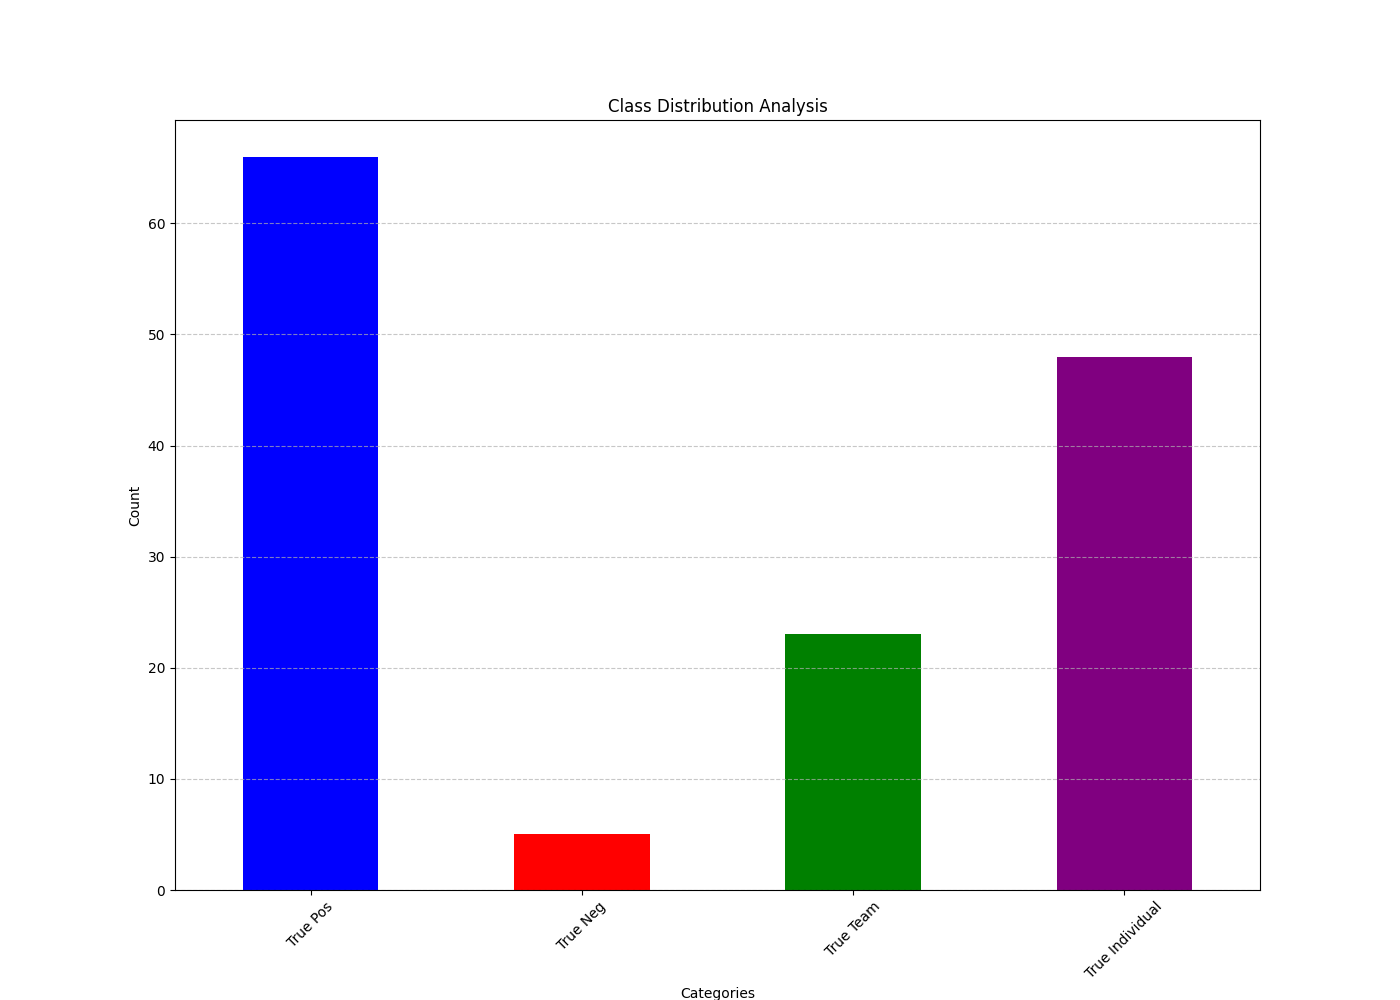
\includegraphics[width=1.2\textwidth]{class_distribution_plot.png}}
  \caption{Class Distribution Analysis per Label}
  \label{fig:class_distribution}
\end{figure}

The following insights can be gathered from the class distribution analysis:
\begin{itemize}
  \item \emph{True Pos} is the most frequent labels, significantly higher than the others while its counterpart, \emph{True Neg} has very few occurences. This
  suggests an imbalance in the sentiment label classes. This large gap between the two might be indicative of a bias towards positive sentiment in the dataset.
  \item Similarly, \emph{True Individual} appears more frequently than \emph{True Team} meaning individual-focused statements are more common in the dataset. The
  imbalance between these two label classes suggests that more statements are focused on individuals rather than teams which could indicate bias or be reflective 
  of the nature of the dataset, implying that, the media focuses on the individual over groups.
  \item A classifier model trained on this dataset may struggle to predict the less frequent classes such as \emph{True Neg}. To avoid potential consequences, the 
  model might need data balancing techniques such as upsampling the minority class or using weighted loss functions in the model in addition to the existing dataset. 
\end{itemize}

\section{Baselines}
% What baselines we chose

\section{Relevant Documents}
% Link to Codabench Page
% Link to Google Slide

\end{document}